% ORIGIN CVPR working draft.
% The latest released official kit at the time of writing is CVPR 2026.
% Replace cvpr.sty/ieeenat_fullname.bst and verify all policy details when the
% CVPR 2027 author kit is released.
\documentclass[10pt,twocolumn,letterpaper]{article}

\usepackage[review]{cvpr}
\usepackage{amsmath,amssymb}
\usepackage{booktabs}
\usepackage{enumitem}
\usepackage{microtype}
\usepackage{array}
\usepackage{multirow}
\usepackage{xspace}

\definecolor{cvprblue}{rgb}{0.21,0.49,0.74}
\usepackage[pagebackref,breaklinks,colorlinks,allcolors=cvprblue]{hyperref}
\usepackage[capitalize,nameinlink]{cleveref}

\def\paperID{*****}
\def\confName{CVPR}
\def\confYear{2027}

\newcommand{\method}{\textsc{Origin}\xspace}
\newcommand{\NA}{\textemdash}
\newcommand{\R}{\mathbb{R}}
\DeclareMathOperator*{\argmax}{arg\,max}

\title{Every Threshold Has a Place: Conserved Spatial Evidence\\
Ledgers for Auditable Ordinal Vision}

\author{Anonymous Authors}

\begin{document}
\maketitle

\begin{abstract}
Disease severity is ordinal and is often supported by small, spatially
distributed findings, yet most grading networks first collapse an image to a
global vector and explain the resulting decision afterward.  We introduce
\method, an architecture whose only image-dependent prediction input is a
conserved, boundary-indexed spatial evidence ledger.  A multiscale
convolutional encoder emits bounded nonnegative atoms for adjacent severity
transitions; prerequisite compilation makes higher-severity atoms support
their lower thresholds.  Summing the ledger produces four transition
parameters, decoded in our primary implementation by a pure-birth generator
into a normalized five-grade posterior.  Removing any ledger group and
replaying the same deterministic decoder gives an exact frozen-ledger internal
intervention, without gradients, pixel replacement, re-encoding, or attention
renormalization.  This guarantee belongs to the conserved ledger, not uniquely
to the matrix exponential: an explicitly defined sequential-hazard decoder
shares it, whereas the CTMC alone supplies a homogeneous shared-clock semigroup
across exposure horizons.  On locked, patient-grouped 10-fold EyePACS outer
cross-validation ($N=35{,}126$ pooled out-of-fold predictions), \method obtains
85.99\% accuracy, 0.8153 quadratic weighted kappa (QWK), 0.1963 discrete
MAP-grade mean absolute error (MAE), and 0.2496 posterior-expected-grade MAE;
fold accuracy is
$85.99\!\pm\!0.44$\%.  On complete 5-fold APTOS outer cross-validation, it
obtains 84.87\% accuracy, 0.9118 QWK, and 0.1936 MAP-grade MAE.
In a protocol frozen before its ten trainings but after EyePACS fold~9 had
already been observed, a retrospective study finds that a pooled continuation-ratio
control obtains 86.40\% accuracy
versus 85.66\% for \method and reduces MAP-grade MAE by 0.0145 (paired
patient-cluster 95\% CI $[0.0017,0.0274]$), but worsens ECE by 0.0273
($[0.0198,0.0357]$).  Fine-scale evidence alone loses 1.97 accuracy points
($[1.08,2.88]$).  Thus the present evidence supports accurate grading and
exact ledger replay, but not an accuracy advantage of the factorization,
pixel causality, or lesion semantics.
\end{abstract}

\section{Introduction}
\label{sec:intro}

Diabetic retinopathy (DR) is a common complication of diabetes and a major
cause of preventable vision loss; an estimated 103 million adults had DR in
2020, with the burden projected to rise substantially by 2045
\cite{teo2021global}.  Clinical screening assigns an ordered severity grade
from no apparent DR through proliferative DR \cite{wilkinson2003severity}.
This ordering is not cosmetic: confusing neighboring stages and skipping
several stages represent different errors, and severe grades are supported by
increasing or qualitatively stronger retinal findings.

Modern ordinal methods encode order through cumulative thresholds
\cite{cao2020coral,shi2023corn}, soft targets \cite{diaz2019sord}, structured
embeddings \cite{li2021poe,lei2024core}, contrastive margins
\cite{pitawela2025cloc,saleem2025hybrid}, or label sequences
\cite{wang2023ord2seq,yu2025aordr}.  These methods improve the output geometry,
but their decision is normally made from a pooled representation.  Conversely,
post-hoc maps such as Grad-CAM \cite{selvaraju2017gradcam} may localize a
prediction, but are not the prediction mechanism; moreover, parameter and
data randomization tests reveal that some popular saliency variants can be
insensitive to the learned model \cite{adebayo2018sanity}.  Even intrinsically
spatial models usually aggregate local scores into class logits
\cite{javed2022additive,donteu2024sparse} or attention tokens
\cite{shiku2025satomil}.  What remains underexplored is an ordinal object that
addresses evidence at every adjacent threshold and can be intervened on
without changing unselected computation.  We seek three properties together:

\begin{enumerate}[leftmargin=*,itemsep=1pt,topsep=2pt]
  \item a valid joint posterior over ordered grades;
  \item a prediction path composed exclusively of spatial evidence; and
  \item an intervention whose reported effect is exactly the effect inside that
        same prediction circuit.
\end{enumerate}

We propose \method to couple these properties through a conserved ordinal
evidence ledger.  The model converts multiscale feature cells into bounded,
nonnegative contributions to the four adjacent transitions of a five-grade
scale.  These entries are the complete image-dependent input to a declared
ordinal decoder.  Our primary decoder is a pure-birth CTMC, but the ledger
contract is decoder-agnostic: subtraction followed by the same deterministic
decoder is exact for either the CTMC or a sequential-hazard control.  The
explanation is therefore not a visualization of a hidden classifier; it is an
addressable decomposition of the quantity from which the posterior is
computed.

Our contributions are:
\begin{itemize}[leftmargin=*,itemsep=1pt,topsep=2pt]
  \item \textbf{Boundary-indexed conserved evidence.}  \method makes a
  nonnegative receptive-field-indexed ledger the exclusive image-dependent
  input to every ordinal threshold; no pooled classifier or prediction bypass
  exists.  A null-simplex head, prerequisite compiler, and conservation law
  make evidence cumulative, bounded, and resolution independent.
  \item \textbf{Exact grouped ledger interventions.}  Deleting or retaining
  declared ledger groups and replaying the identical decoder gives the literal
  posterior change under that frozen-ledger intervention; no backward pass,
  pixel replacement, or renormalization is involved.
  \item \textbf{Explicit decoder contracts.}  Both the CTMC and matched
  sequential-hazard decoder yield normalized fixed-horizon posteriors whose
  cumulative tails are coordinatewise monotone in the rates, as well as exact
  ledger replay.  The CTMC-specific property is a homogeneous
  shared-clock Markov semigroup across horizons, whose utility is not tested by
  one endpoint grade per image.
  \item \textbf{Locked ordinal evaluation.}  We report complete 5-fold APTOS
  and patient-grouped 10-fold EyePACS outer cross-validation, including QWK,
  MAE, calibration, balanced accuracy, and minority-grade recall rather than
  accuracy alone.  A separate ten-arm, patient-paired fold-9 mechanism study
  reports both favorable and falsifying evidence for the architectural
  components without blending it into the full-CV estimate.
\end{itemize}

\begin{figure*}[t]
  \centering
  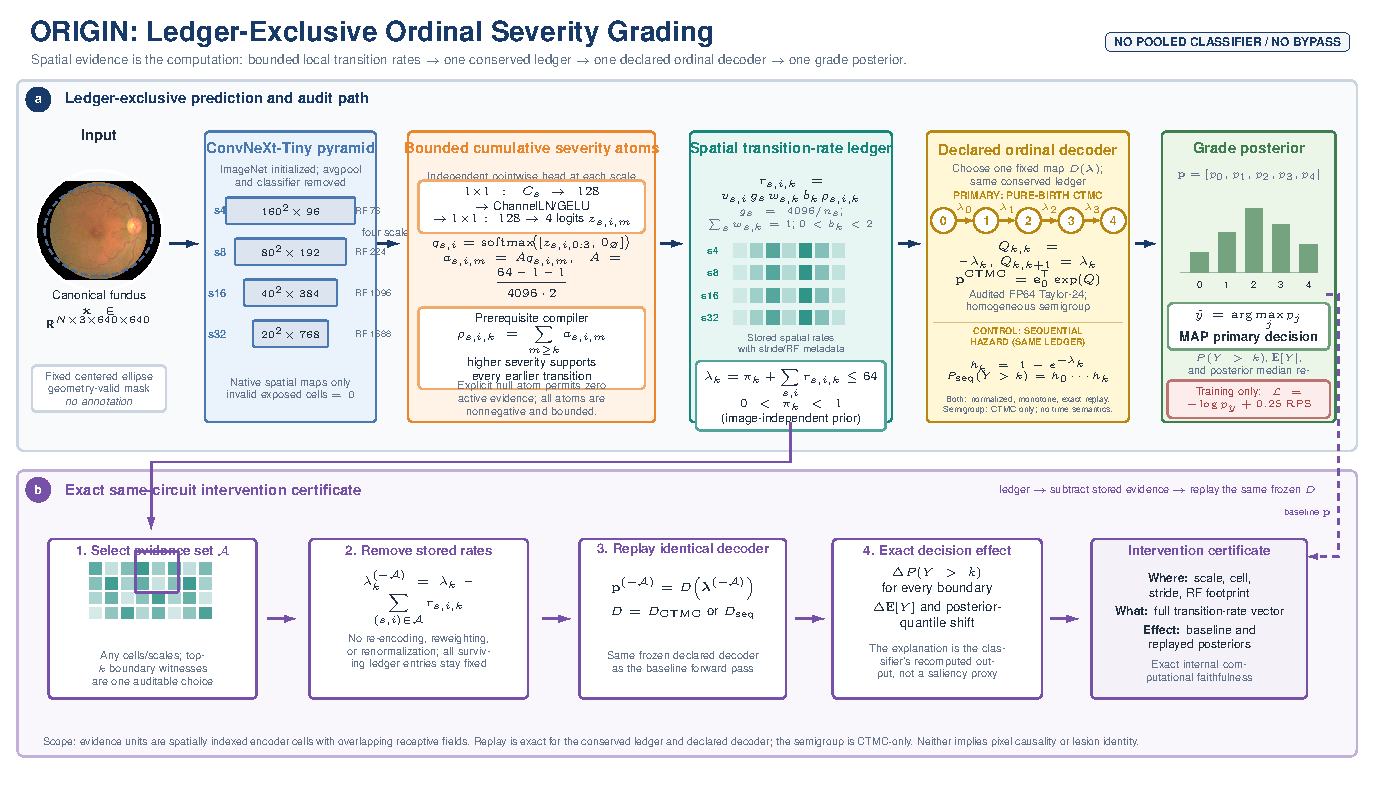
\includegraphics[width=\textwidth]{../output/pdf/ORIGIN_v3_architecture.pdf}
  \caption{\textbf{ORIGIN architecture.}  A canonical fundus image is encoded
  into four native ConvNeXt feature fields.  Pointwise heads produce bounded
  severity atoms; prerequisite compilation and a conserved ledger yield four
  nonnegative adjacent-state rates.  The primary pure-birth decoder maps those
  rates to the only grade posterior.  For an intervention, selected stored
  rates are subtracted and the identical declared decoder is replayed.  The
  certificate is exact for the model's frozen ledger, not a claim of pixel
  causality or lesion identity; the replay contract also holds for the
  same-ledger sequential-hazard control.}
  \label{fig:architecture}
\end{figure*}

\section{Related Work}
\label{sec:related}

\paragraph{Ordinal image prediction.}
Deep ordinal learning has been formulated as unimodal output distributions
\cite{beckham2017unimodal}, soft labels \cite{diaz2019sord}, rank-consistent
cumulative or conditional classifiers \cite{cao2020coral,shi2023corn,
jenkinson2021condor}, probabilistic
embeddings \cite{li2021poe}, and consistent representations
\cite{lei2024core}.  Ord2Seq generates a label sequence
\cite{wang2023ord2seq}; CLOC learns boundary-dependent contrastive margins
\cite{pitawela2025cloc}; and recent DR systems combine ordinal learning with
contrastive objectives \cite{saleem2025hybrid} or autoregressive diffusion
\cite{yu2025aordr}.  Directed ordinal diffusion regularization shapes a feature
space according to a forward disease trajectory \cite{chen2026dodr}.  In
contrast, our pure-birth construction is an \emph{image-level algebraic
decoder}: its unit exposure is not elapsed biological time, it does not model a
patient's longitudinal progression, and it produces the joint posterior in one
matrix exponential.

\paragraph{Spatial and intrinsic interpretation.}
Gradient maps \cite{selvaraju2017gradcam} explain a trained predictor after the
fact.  Lesion-aware transformers jointly grade DR and discover regions from
image labels, but their localization remains a learned auxiliary mechanism
\cite{sun2021lat}.  Concept bottlenecks expose semantic intermediate variables
\cite{koh2020cbm}, but normally require concept supervision and do not by
themselves provide local evidence.  Additive MIL makes regional contributions
to a pooled prediction explicit \cite{javed2022additive}.  Sparse disease
grading adapts BagNet to produce fine, faithful class-evidence fields for small
DR lesions \cite{donteu2024sparse}, while ordinal MIL uses selective
aggregation tokens for threshold-specific evidence \cite{shiku2025satomil}.
These are closest in spirit, but \method differs in the object being
decomposed: each local entry is a nonnegative vector of adjacent-state
\emph{generator rates}, and the same stored entries can be removed and replayed
through the exact ordinal decoder.

\paragraph{Generator view.}
For a continuous-time Markov chain, a valid generator defines a stochastic
transition matrix through the matrix exponential \cite{le2022ctmc}.  Li and
Lin superpose transition rates derived from specialized classifiers and use
the CTMC equilibrium distribution to combine their predictions
\cite{li2017ctmc}.  DiDiCM instead learns a discrete diffusion process over
general class labels \cite{belhasin2026didicm}.  \method differs from both: its
primary forward-only pure-birth chain maps a conserved local evidence ledger to
a finite-time ordinal posterior.  We use the generator as a constrained
probability layer rather than as a temporal disease model.  Importantly, exact
ledger replay is not CTMC-specific; we compare a sequential-hazard map applied
to the identical ledger.  The distinguishing CTMC contract is instead the
homogeneous semigroup $\exp((t+r)Q)=\exp(tQ)\exp(rQ)$ across exposure horizons
\cite{le2022ctmc}.  Scaling and squaring is a standard route to stable matrix
exponentials \cite{higham2005scaling}; our small structured generator permits a
fixed, audited FP64 implementation.

\section{Method}
\label{sec:method}

\subsection{Problem and design contract}

Let $x_n$ be an image and $y_n\in\{0,\ldots,K-1\}$ its ordered grade.  For DR,
$K=5$ and there are $B=K-1=4$ adjacent boundaries.  We require that every
image-dependent quantity reaching the posterior be addressable by scale and
cell, nonnegative, and exactly conserved under aggregation.  No global pooled
classifier, auxiliary logit, or residual decision route is allowed.  The full
forward pass is summarized in \cref{fig:architecture}.

\subsection{Multiscale spatial fields}

After cropping the dominant retinal field, we resize to $640\!\times\!640$ and
apply ImageNet normalization.  An ImageNet-pretrained ConvNeXt-Tiny
\cite{liu2022convnext}, with its pooling and classifier removed, exposes four
native feature fields $F_s$:

\begin{table}[t]
  \centering
  \caption{Native evidence fields for a $640\times640$ input.  RF denotes the
  declared theoretical receptive-field footprint used in certificates.}
  \label{tab:fields}
  \setlength{\tabcolsep}{4.2pt}
  \begin{tabular}{@{}lrrrr@{}}
    \toprule
    Scale & Grid & Channels & Stride & RF (px) \\
    \midrule
    $s4$  & $160^2$ & 96  & 4  & 76 \\
    $s8$  & $80^2$  & 192 & 8  & 224 \\
    $s16$ & $40^2$  & 384 & 16 & 1096 \\
    $s32$ & $20^2$  & 768 & 32 & 1688 \\
    \bottomrule
  \end{tabular}
\end{table}

A fixed centered elliptical mask encodes only retinal support; it is not an
annotation.  A feature cell is valid when at least half of its pooled input
support lies inside the ellipse.  Invalid exposed cells are zeroed after the
encoder.  Each scale has a separate pointwise head
$1\!\times\!1\rightarrow128$, channel LayerNorm, GELU, and
$1\!\times\!1\rightarrow B$.  There is no cross-cell operation in these
heads.

\subsection{Bounded atoms and prerequisite compilation}
\label{sec:atoms}

For valid cell $u$ at scale $s$, the head emits logits
$z_{nsu}\in\R^B$.  Appending a fixed zero-logit null state gives
\begin{equation}
q_{nsum}=
\frac{\exp z_{nsum}}
{1+\sum_{j=0}^{B-1}\exp z_{nsuj}},
\qquad
a_{nsum}=Aq_{nsum},
\label{eq:null-simplex}
\end{equation}
for atom $m\in\{0,\ldots,B-1\}$.  Hence $a_{nsum}\geq0$ and
$\sum_m a_{nsum}<A$; the remaining mass is explicit ``no severity evidence.''

A higher-transition atom can serve as cumulative evidence for prerequisite
lower transitions.  We encode this inductive bias before any image-level
aggregation:
\begin{equation}
c_{nsuk}=\sum_{m=k}^{B-1}a_{nsum},
\qquad k=0,\ldots,B-1.
\label{eq:compiler}
\end{equation}
Thus $c_{nsu0}\geq\cdots\geq c_{nsu,B-1}\geq0$.  The atom index is a learned
severity-transition type, not a named clinical lesion; semantic lesion claims
require separate validation.

\subsection{Conserved transition-rate ledger}
\label{sec:ledger}

Let $V_{nsu}\in\{0,1\}$ mark valid cells and
$N_{ns}=\sum_u V_{nsu}$.  With reference count $R=4096$, define
\begin{equation}
g_{ns}=\begin{cases}R/N_{ns},&N_{ns}>0,\\0,&N_{ns}=0.\end{cases}
\label{eq:geometry}
\end{equation}
For each boundary, scale weights form a simplex,
$w_{sk}=\exp\alpha_{sk}/\sum_t\exp\alpha_{tk}$, while
$b_k=2\sigma(\beta_k)$ calibrates that boundary.  The stored contribution is
\begin{equation}
\ell_{nsuk}=V_{nsu}\,g_{ns}\,w_{sk}\,b_k\,c_{nsuk}\geq0,
\label{eq:local-rate}
\end{equation}
and the image rate is exactly
\begin{equation}
\lambda_{nk}=\pi_k+\sum_s\sum_u\ell_{nsuk},
\qquad \pi_k=\sigma(\nu_k)\in(0,1).
\label{eq:ledger}
\end{equation}
The prior $\pi_k$ is image independent.  All image-dependent influence on the
posterior is contained in the spatial ledger $\ell$.

\paragraph{Resolution-independent bound.}
Let the decoder ceiling be $C=64$, the prior cap $P=1$, the calibration cap
$b_{\max}=2$, and the roundoff reserve $\delta=1$.  We set
\begin{equation}
A=\frac{C-P-\delta}{Rb_{\max}}=\frac{62}{8192}.
\label{eq:atom-cap}
\end{equation}
Because geometry normalization cancels the number of valid cells and
$\sum_s w_{sk}=1$,
\begin{equation}
0<\lambda_{nk}<P+Rb_{\max}A=63<C.
\label{eq:rate-bound}
\end{equation}
The bound holds regardless of feature-map resolution, preventing evidence from
growing merely because a field contains more cells.

\subsection{Pure-birth ordinal posterior}
\label{sec:generator}

The boundary rates parameterize a $K\times K$ upper-bidiagonal generator
\begin{equation}
Q_{k,k}=-\lambda_k,\qquad Q_{k,k+1}=\lambda_k,
\qquad Q_{K-1,K-1}=0.
\label{eq:generator}
\end{equation}
Starting in state zero, the unit-exposure posterior is
\begin{equation}
\mathbf p=e_0^\top\exp(Q),
\qquad p_j=P(Y=j\mid x).
\label{eq:posterior}
\end{equation}
Since $Q$ is a valid generator, $\mathbf p$ is nonnegative and sums to one.
We compute \cref{eq:posterior} in FP64 with a degree-24 Taylor
scaling-and-squaring routine.  For a decoder batch, let
$\eta=\max_n\lVert Q_n\rVert_\infty$ and
$s=\max\{0,\lceil\log_2(\eta/0.5)\rceil\}$.  We evaluate each Taylor
polynomial at $Q_n/2^s$ and square the result $s$ times.  No posterior clipping
or renormalization is applied.
The unit exposure is simply a fixed decoder convention; $\lambda$ is latent
ordinal evidence, not biological time.

The model exposes $P(Y>k)=\sum_{j=k+1}^{K-1}p_j$, expected grade
$E[Y]=\sum_jjp_j$, posterior quantiles, and MAP.  The frozen primary decision
is $\hat y=\argmax_jp_j$.  Increasing all rates componentwise advances the
chain in first-order stochastic order, so cumulative probabilities, expected
grade, and posterior quantiles are monotone.  MAP itself need not change
monotonically and is not claimed to do so.

\subsection{Decoder scope and sequential-hazard control}
\label{sec:decoder-scope}

To isolate the ledger from its primary decoder, we apply adjacent conditional
hazards to the \emph{identical} stored rates.  At horizon $t$, let
\begin{equation}
h_k(t)=1-\exp(-t\lambda_k),\qquad
P_{\mathrm{seq}}(Y>k)=\prod_{j=0}^{k}h_j(t).
\label{eq:sequential-tails}
\end{equation}
The corresponding normalized posterior is
\begin{equation}
p^{\mathrm{seq}}_y=
\begin{cases}
(1-h_y)\prod_{j<y}h_j,&y<K-1,\\
\prod_{j=0}^{K-2}h_j,&y=K-1.
\end{cases}
\label{eq:sequential-posterior}
\end{equation}
Both decoders are normalized and coordinatewise monotone on the deployed
bounded rate domain at the fixed horizon $t=1$; both inherit exact deletion
replay from the ledger.  A seeded numerical inversion audit over 64 sampled
interior-simplex targets found maximum posterior reconstruction errors of
$2.08\times10^{-12}$ (CTMC) and $1.95\times10^{-16}$ (sequential).  This
supports coverage of those tested targets, not universal representation of
every interior posterior under finite rate bounds, and gives no evidence of a
fixed-horizon expressiveness advantage for the CTMC in the sampled audit.

The CTMC-specific guarantee is cross-horizon: its transition kernel
$P(t)=\exp(tQ)$ shares one clock and obeys the homogeneous Markov semigroup
$P(t+r)=P(t)P(r)$.  The natural restartable kernel induced by
\cref{eq:sequential-posterior} does not satisfy this identity in general.  Our
cross-sectional labels observe only one endpoint, so we treat this as a
mathematical contract, not an empirically validated disease-progression claim.

\paragraph{Scope of guarantees.}
Exclusivity, nonnegative conservation, boundary addressability, and exact
grouped replay are \emph{ledger-wide}.  Normalization and coordinatewise
monotonicity hold for \emph{both declared decoder instantiations}.  The
homogeneous shared-clock semigroup is \emph{CTMC-specific}.  We make no claim
that the last property improves cross-sectional grading.

\subsection{Exact frozen-ledger intervention}
\label{sec:intervention}

Let $D_\theta$ denote either declared deterministic decoder above.  For any
selected ledger set $S$ (cells, scales, or both), deletion is
\begin{equation}
\lambda^{(-S)}_{nk}=\lambda_{nk}-
\sum_{(s,u)\in S}\ell_{nsuk},
\qquad
\mathbf p^{(-S)}=D_\theta(\lambda^{(-S)}_n).
\label{eq:intervention}
\end{equation}
The complementary retain-only replay is
$\lambda^{(+S)}_{nk}=\pi_k+\sum_{(s,u)\in S}\ell_{nsuk}$ and
$\mathbf p^{(+S)}=D_\theta(\lambda^{(+S)}_n)$.
The encoder, support masks, geometry factors, scale weights, and all surviving
ledger entries remain fixed.  Therefore the reported change
$\Delta P(Y>k)$ or $\Delta E[Y]$ is the literal difference between the baseline
computation and the internally intervened computation.  The identity follows
from ledger conservation and deterministic replay; it is not unique to
$\exp(Q)$.  This avoids a common confound of pixel occlusion: replacing image
content and re-encoding can create out-of-distribution artifacts and can change
every feature.

Each certificate stores the scale, cell coordinate, receptive-field footprint,
full boundary-rate vector, baseline posterior, replayed posterior, and decision
effect.  Overlapping receptive fields mean that cells are computational units,
not disjoint pixel segments.  Accordingly, exactness establishes
\emph{computational faithfulness inside \method}; it does not by itself prove
pixel causality, lesion identity, clinical sufficiency, or clinical necessity.
For budget-matched audits we define the nominal stride-area cost
$A_{\mathrm{nom}}(S)=\sum_{(s,u)\in S}\operatorname{stride}_s^2$.  This is an
additive multiscale addressability cost, not unique pixel coverage or the union
area of overlapping receptive fields.

\subsection{Objective}

We train the generated posterior with negative log likelihood and the ranked
probability score (RPS), a proper score sensitive to ordinal distance
\cite{epstein1969rps,gneiting2007proper}:
\begin{equation}
\begin{aligned}
\mathcal L={}&-\frac1N\sum_n\log p_{n,y_n} \\
&+\frac{0.25}{N(K-1)}\sum_{n,k}
\left(P(Y_n>k)-\mathbf{1}[y_n>k]\right)^2.
\end{aligned}
\label{eq:loss}
\end{equation}
Here $\mathbf{1}$ is implemented as a binary target; no separate head is used.
There is no class weighting, oversampling, auxiliary classifier, or active
evidence-budget penalty in the frozen model.

\section{Experiments}
\label{sec:experiments}

\subsection{Datasets and locked protocol}

\paragraph{EyePACS.}
The Kaggle 2015 DR training set contains 35,126 images with grade counts
$[25{,}810, 2{,}443, 5{,}292, 873, 708]$ \cite{kaggle2015eyepacs}.  We use
10-fold outer cross-validation grouped by patient identifier parsed from the
filename; left and right eyes from one patient remain together in outer and
inner partitions.

\paragraph{APTOS 2019.}
APTOS contains 3,662 images with grade counts
$[1{,}805,370,999,193,295]$, acquired under heterogeneous cameras and imaging
conditions \cite{aptos2019}.  Because patient identifiers are unavailable, we
use image-stratified 5-fold outer cross-validation and state this weaker split
explicitly.

Within each outer training pool, 10\% is reserved as an inner validation split.
Training and checkpoint choice use only the inner split.  After selection is
finalized, the checkpoint is evaluated on the locked outer fold; a second
deterministic pass exports per-image probabilities for auditing.  Neither pass
affects training or selection.  Architecture and hyperparameters were developed
on fixed inner-validation splits.  The bounded V3 architecture was frozen on
10 September 2026; the immutable full-CV launcher, split policy, and selection
rule were frozen on 22 September before the 15 outer-fold evaluations.  Thus per-fold
checkpointing is nested, but architecture selection was not independently
repeated inside every outer fold.  No outer test fold was used for checkpoint
selection.  The final EyePACS OOF audit contains 35,126 unique images from
17,563 patients (two eyes each), with no patient crossing an outer fold.

\subsection{Implementation and metrics}

We optimize with AdamW (encoder LR $10^{-4}$, new-head LR $5\times10^{-4}$,
weight decay $10^{-5}$), batch size 8, and gradient clipping at 5.  The encoder
is frozen for two epochs and then jointly fine-tuned.  ReduceLROnPlateau monitors
validation loss (factor 0.2, patience 5, minimum LR $10^{-6}$).  APTOS runs for
at most 35 epochs with early-stop patience 12; EyePACS uses 75 and 15.  The
checkpoint rule is lexicographic: validation accuracy, then QWK, then lower
loss.  Training uses horizontal/vertical flips, rotations up to $30^\circ$, and
moderate color jitter.  AMP is used for the encoder and heads; the generator is
FP64.  Runs used Python 3.11, PyTorch 2.5.1, and a 32-GB Tesla V100.

We report accuracy, discrete MAP-grade MAE, posterior-expected-grade MAE, QWK,
balanced accuracy, macro-F1, 15-bin top-label expected calibration error (ECE),
confusion matrices, and per-grade recall.  Fold spread is the sample standard
deviation.  Class MAP is the primary decision rule fixed before looking at
outer tests; alternative decoders are not selected post hoc.

\paragraph{Numerical reference audit.}
The deployed FP64 Taylor scaling-and-squaring decoder was compared with an
independent 90-decimal-digit \texttt{mpmath.expm} reference on 138 seeded random
and adversarial rate vectors in $[0,64]^4$, plus 12 independent
finite-difference gradient cases.  The audit passed without clipping or
renormalization: maximum absolute posterior, row-sum, and absolute-gradient
errors were respectively below $1.5\times10^{-14}$,
$1.7\times10^{-14}$, and $1.4\times10^{-15}$.

\paragraph{Artifacts and verification.}
An automated release manifest binds all 15 selected checkpoints and 15
compressed split-membership tables to SHA-256 hashes, split signatures,
implementation signatures, and the source commit.  The anonymous release gate
also requires OOF posteriors, deterministic split construction, intervention
records, metric/bootstrap scripts, and restart provenance to pass checksums
before any newly added acceptance-audit table is reported.  Membership
identities are hashed and no fundus pixels are redistributed; image access
remains subject to the source dataset licenses.

\subsection{Required comparisons}

The external numbers in \cref{tab:main-results} are literature-reported rather
than matched reimplementations.  Exact fold membership and checkpoint-selection
artifacts are unavailable for CORE and Ord2Seq, while the Hybrid study does not
publish fold assignments or fold-wise dispersion.  To avoid mixing estimators,
we report both our primary discrete MAP-grade MAE and a posterior-expected-grade
MAE matched to Ord2Seq's definition.  Protocol and preprocessing differences
can still move results substantially; therefore the external rows contextualize,
but do not establish, superiority.  Studies using materially different fold
counts or split construction are omitted rather than juxtaposed numerically.
Our matched fold-9 study trains pooled multiscale softmax, cumulative-logit,
and conditional continuation-ratio heads; a same-ledger sequential-hazard
decoder; direct-simplex and independent-sigmoid atom variants; NLL-only,
fine-only, and coarse-only variants; and a contemporaneously rerun full
\method model.  These pooled ordinal forms are matched controls, not exact
reimplementations of published CORAL or CORN systems.  Matched CLOC and
sparse/additive local models were not part of that retrospective suite.  A
separately frozen acceptance matrix now reserves comparisons against the
same-ledger hazard, pooled continuation ratio, and matched in-repo analogues of
ordinal Additive MIL and a nonnegative sparse local-logit model across matched
folds and seeds.  These
are controlled architectural analogues, not claims of reproducing the original
authors' training code.  Their results are withheld until the complete release
gate passes.

\subsection{Retrospective matched fold-9 mechanism study}
\label{sec:ablation-protocol}

We separately study mechanisms on EyePACS outer fold~9.  The final V3
architecture predates full CV, but the mechanism protocol was added on 26
September after the full-CV aggregate and fold~9 had been
observed.  This is therefore retrospective evidence, not a confirmatory test.
The split contains 28,456 training, 3,162
inner-validation, and 3,508 locked outer-test images.  The test images form
1,754 patient clusters (both eyes remain paired).  Ten independently trained
variants use the same patient split, ImageNet initialization policy,
augmentation, optimizer, dedicated training-stream seed, checkpoint rule, and
maximum 75-epoch training policy.  Inner validation alone selects each
checkpoint.  After all ten training-completion markers existed, one
nonadaptive suite-level release evaluated every selected checkpoint on the
locked outer fold.  The study uses one training seed, so its patient-cluster
intervals quantify test-cohort sampling variation conditional on fitted models,
not training variability.

\section{Results}
\label{sec:results}

\begin{table*}[t]
  \centering
  \caption{Outer-cross-validation results.  ORIGIN values are pooled
  out-of-fold predictions from our locked protocol; external values are quoted
  from the cited primary papers and are not matched reruns.  Reported protocols
  are not split-identical.  $^{\mathrm{M}}$ denotes discrete MAP-grade MAE and
  $^{\mathrm{E}}$
  posterior-expected-grade MAE; unmarked external values retain the estimator
  reported by their authors.  Higher accuracy/QWK and lower MAE are better.}
  \label{tab:main-results}
  \small
  \setlength{\tabcolsep}{4pt}
  \begin{tabular}{@{}lclccccl@{}}
    \toprule
    Dataset & Protocol & Method & Acc. (\%) & QWK & MAE (est.) & Status & Source \\
    \midrule
    \multirow{4}{*}{EyePACS}
      & reported 10-fold & CORE+POE (VGG-19) & 84.3 & \NA & 0.2718
      & reported & \cite{lei2024core} \\
      & reported 10-fold & Ord2Seq (PVTv2-B1) & $84.2\!\pm\!0.5$ & \NA &
      $0.25\!\pm\!0.07^{\mathrm{E}}$ & fold mean & \cite{wang2023ord2seq} \\
      & reported 10-fold & Hybrid Eff.-V2S & 83.8 & \NA & 0.21
      & reported & \cite{saleem2025hybrid} \\
      & patient 10-fold & \textbf{ORIGIN} & 85.99 & 0.8153 &
      $0.1963^{\mathrm{M}}/0.2496^{\mathrm{E}}$
      & pooled OOF & ours \\
    \midrule
    APTOS
      & image 5-fold & \textbf{ORIGIN} & 84.87 & 0.9118 &
      $0.1936^{\mathrm{M}}/0.2168^{\mathrm{E}}$
      & pooled OOF & ours \\
    \bottomrule
  \end{tabular}
  \par\smallskip
  \parbox{0.94\textwidth}{\centering Matched controls on one previously
  observed EyePACS fold are summarized in \cref{sec:ablations} and reported
  fully in the supplement; they do not replace the complete-CV estimate or
  establish population-level superiority.}
\end{table*}

\subsection{Grading performance}

On complete APTOS outer CV, \method obtains
$84.872\!\pm\!0.508$\% fold-mean accuracy, $0.9117\!\pm\!0.0073$ QWK, and
$0.1936\!\pm\!0.0072$ MAP-grade MAE.  Pooled out-of-fold accuracy is 84.872\%,
with 63.67\% balanced accuracy, 0.6438 macro-F1, and 0.0502 ECE.  The pooled
posterior-expected-grade MAE is 0.2168 (fold mean
$0.2168\!\pm\!0.0080$).  The small accuracy spread indicates stable overall
grading across the five partitions.

On complete EyePACS outer CV, pooled out-of-fold performance is 85.988\%
accuracy, 0.8153 QWK, 0.1963 MAP-grade MAE, 57.56\% balanced accuracy,
0.6223 macro-F1, and 0.0288 ECE.  Fold-mean accuracy is
$85.988\!\pm\!0.442$\%; fold-mean QWK and MAP-grade MAE are
$0.8152\!\pm\!0.0189$ and $0.1963\!\pm\!0.0113$.  The estimator-matched
posterior-expected-grade MAE is 0.2496 (fold mean
$0.2496\!\pm\!0.0143$), essentially the same as Ord2Seq's reported
$0.25\!\pm\!0.07$.  Among the audited studies labelled as 10-fold EyePACS
evaluations, our accuracy is descriptively 1.69 points above CORE+POE (84.3\%)
and 1.79 points above Ord2Seq-PVT (84.2\%).  These are unpaired,
protocol-heterogeneous differences, not matched evidence of superiority.

\begin{table}[t]
  \centering
  \caption{Per-grade recall (\%) from complete pooled outer-fold predictions.}
  \label{tab:recall}
  \setlength{\tabcolsep}{4pt}
  \begin{tabular}{@{}lrrrrr@{}}
    \toprule
    Dataset & G0 & G1 & G2 & G3 & G4 \\
    \midrule
    EyePACS (10/10) & 96.91 & 28.53 & 71.69 & 35.28 & 55.37 \\
    APTOS (5/5)    & 98.78 & 50.27 & 91.89 &  7.25 & 70.17 \\
    \bottomrule
  \end{tabular}
\end{table}

\paragraph{Long-tail behavior.}
\Cref{tab:recall} prevents headline accuracy from hiding failure modes.
The no-DR class is recognized reliably, but mild and severe NPDR remain hard.
On EyePACS, 1,335 of 2,443 grade-1 images are predicted as grade 0 and 500 of
873 grade-3 images as grade 2.  Overall, 94.96\% of predictions are exact or
adjacent, while 5.04\% differ by at least two grades.  APTOS grade-3 recall is
only 7.25\%: 136 of 193 grade-3 images are predicted as grade 2.  These are
major current limitations, not evidence that the ordinal mechanism has solved
imbalance.  Importantly, the frozen objective intentionally uses the unweighted
population likelihood; targeted imbalance methods must be compared without
compromising calibration or the ledger semantics.

\subsection{Structural identity versus empirical utility}

The intervention identity in \cref{eq:intervention} is structural.  The ten
EyePACS folds archive 40 inner-validation certificates (four per fold): the
maximum stored-ledger partition error is exactly zero and the maximum total-rate
replay error is $5.56\times10^{-17}$.  The present sample is not
grade-stratified---34 of 40 cases are grade 0---and no single-cell deletion
changes MAP.  Moreover, 29 of 40 selected witnesses come from the coarse $s16$
or $s32$ fields, and mean $|\Delta E[Y]|$ is only 0.00389.  These artifacts
verify replay arithmetic; they do \emph{not} demonstrate useful fine-grained
localization.  We therefore separate the proved \emph{arithmetic identity of
frozen-ledger replay} from the still-open empirical question of whether learned
witnesses are local, useful, or semantically aligned.

\paragraph{IDRiD mask association.}
All ten independently inner-selected EyePACS outer-fold checkpoints evaluate
the 81-image IDRiD segmentation subset \cite{porwal2020idrid}, with no IDRiD
training, tuning, or selection.  We form the official MA/HE/EX/SE union; apply
the image-derived dominant-FOV crop to image and masks; and resize the image
bilinearly and mask by nearest neighbor.  A native-lattice bin is positive iff
it contains any mask pixel; its score is the stored \texttt{local\_rate\_map}
at true-grade boundary $b(y)=\min\{\max(y-1,0),3\}$.  AP is computed per
image$\times$checkpoint$\times$scale, then averaged over checkpoints/scales
within image; inference clusters by image.  Deletion uses 20 seeded,
deterministic nonlesion controls per image, checkpoint, and scale.

V1 fine deletion was exactly count-matched and yielded mask-guided replay lift
$0.0111$ in $|\Delta E[Y]|$ ($[0.0097,0.0125]$).  Its AP and coarse/all-scale
deletion estimates are provisional: AP did not group exact score ties and 14
coarse image$\times$scale cases were under-matched.  A sealed corrective v2
(pending) uses threshold-grouped AP and 20 paired within-image/scale draws of
equal unique lesion/nonlesion counts, matching scale composition, geometry
exposure, and the pre-atom boundary multiplier.  Retinal anatomy and removed
rate mass are not matched; the latter is the outcome.  These are internal
ledger interventions, not pixel deletion, lesion recognition, or clinical
necessity.

\section{Ablations and Falsification Tests}
\label{sec:ablations}

Ablations should be able to falsify, rather than merely decorate, an
architectural claim.  We therefore compare the contemporaneously rerun full
model against nine controls under the frozen protocol in
\cref{sec:ablation-protocol}.  All per-image posteriors, absolute metrics, and
10,000 patient-cluster paired intervals were reproduced independently.  The
complete ten-arm tables are placed in the supplement because this retrospective
single-fold study is mechanism evidence rather than the primary benchmark.

\paragraph{Predictive controls.}
The pooled continuation-ratio model is the strongest grader on this fold:
86.40\% accuracy, 0.8299 QWK, and 0.1861 MAP-MAE, versus 85.66\%, 0.8132,
and 0.2007 for full \method.  Accuracy and QWK intervals include zero, but its
MAP-MAE is lower by 0.0145 ($[-0.0274,-0.0017]$); conversely, ECE is worse by
0.0273 ($[0.0198,0.0357]$).  This performance--calibration--auditability
tradeoff does not establish population-level superiority from one fold.

\paragraph{Scale falsification.}
Fine fields alone are decisively insufficient for grading: relative to full
\method they lose 1.97 accuracy points ($[-2.88,-1.08]$) and 0.0589 QWK
($[-0.084,-0.035]$); grade-4 recall falls from 66.15\% to 21.54\%.  Coarse-only
evidence has the same accuracy point estimate as full \method, with all primary
intervals spanning zero.  This is not equivalence, but it prevents a claim of
demonstrated fine-lesion localization.

\paragraph{Decoder, atoms, and objective.}
The same-ledger sequential-hazard decoder, direct-simplex atoms,
independent-sigmoid atoms, and NLL-only objective all have accuracy, QWK, and
MAP-MAE intervals spanning zero relative to full \method.  Thus this fold does
not show that the CTMC, prerequisite compiler, or RPS improves grading.
Sequential hazards improve ECE by 0.0072 ($[0.0003,0.0137]$).  All variants
contain 27.86--28.07M parameters.  Because this is one retrospective fold, one
seed, and multiple unadjusted comparisons, these are mechanism findings only.

\section{Discussion and Limitations}
\label{sec:discussion}

\paragraph{What is novel.}
The ingredients---ConvNeXt features, nonnegative maps, ordinal decoders,
generators, and proper scores---are established.  The contribution is their
coupling into a boundary-indexed ledger that is the exclusive image path,
cumulative across prerequisites, and exactly group-replayable.  This narrow,
falsifiable claim holds for both declared decoders.

\paragraph{What exactness does not imply.}
Deletion asks what the model would predict without selected stored entries while
survivors remain fixed.  It does not establish pixel causality, lesion identity,
or clinical usefulness.  Coarse receptive fields make this distinction
especially important; pixel masking, external masks, and clinician evaluation
remain complementary.

\paragraph{Data and protocol.}
EyePACS is strongly imbalanced, APTOS lacks patient identifiers, and both use
single noisy competition labels.  Architecture search used a fixed inner split
rather than fully nested hyperparameter selection, so CV estimates performance
of the frozen configuration, not clinical deployment.  External domains and
multi-reader labels are needed.  Two non-finite attempts failed closed and were
rerun unchanged; restart provenance is supplemental.  The revision manifest
hashes checkpoints and split memberships for integrity and disjointness checks;
hashes alone provide neither the artifacts nor executable re-inference.

\paragraph{Model scope.}
The ImageNet-pretrained model is not a medical foundation model.  Evidence
atoms are severity-indexed, not clinical concepts; generalization beyond fundus
grading requires new modalities and datasets.

\paragraph{Potential impact.}
Replay can audit shortcuts only if the pending controlled benchmark passes; it
does not replace clinical judgment.  Rare-grade errors require external
validation, calibration, monitoring, and human oversight.

\section{Conclusion}
\label{sec:conclusion}

\method makes a conserved boundary-indexed ledger the exclusive prediction
input and an exactly replayable audit object.  Complete CV supports competitive
grading; a retrospective fold shows neither an advantage over pooled heads nor
fine-only sufficiency.  Broader claims await the sealed audits.

{\small
  \bibliographystyle{ieeenat_fullname}
  \bibliography{origin_cvpr_refs}
}

\end{document}
